\chapter{Phương pháp thực hiện}
\label{ch:phuong_phap}

Chương này trình bày chi tiết phương pháp triển khai toàn bộ hệ thống, từ kiến trúc tổng thể, chuẩn bị dữ liệu, huấn luyện mô hình cho đến các thuật toán xác định hướng di chuyển, phát hiện vi phạm và nhận diện biển số xe.

\section{Kiến trúc tổng thể của hệ thống}

Hệ thống được thiết kế theo mô hình xử lý đa luồng sử dụng PyQt5 \texttt{QThread} để đảm bảo khả năng xử lý thời gian thực. Quy trình xử lý chính được chia thành các module chuyên biệt tương tác với nhau thông qua Global State quản lý bởi \texttt{VideoThread}.

\begin{figure}[!htbp]
\centering
\begin{tikzpicture}[
    scale=0.85, transform shape,
    node distance=1cm,
    box/.style={rectangle, draw, rounded corners, minimum width=2cm, minimum height=0.6cm, align=center, font=\scriptsize},
    decision/.style={diamond, draw, minimum width=1.2cm, minimum height=0.6cm, align=center, font=\scriptsize, aspect=1.5},
    arrow/.style={->, thick, >=stealth}
]
    % Input
    \node[box, fill=blue!20] (input) {Video Frame};
    
    % YOLO Detection & Tracking
    \node[box, fill=orange!20, below=0.5cm of input] (yolo) {YOLOv8 Detect};
    \node[box, fill=yellow!20, below=0.5cm of yolo] (track) {ByteTrack Tracking};
    
    % Split into 3 branches
    \node[box, fill=green!20, below left=0.8cm and 2.5cm of track] (veh_tracker) {Vehicle Tracker};
    \node[box, fill=cyan!20, below=0.8cm of track] (tl_manager) {Traffic Light Manager};
    \node[box, fill=pink!20, below right=0.8cm and 2.5cm of track] (alpr) {ALPR Pipeline};
    
    % Vehicle Tracker sub-branches
    \node[box, fill=green!30, below left=0.7cm and 0.6cm of veh_tracker] (traj) {Trajectory Analyzer};
    \node[box, fill=green!30, below right=0.7cm and 0.6cm of veh_tracker] (roi_dir) {ROI Direction};
    \node[decision, fill=green!40, below=2cm of veh_tracker] (fusion) {Direction Fusion};
    
    % ALPR sub-pipeline
    \node[box, fill=pink!30, below=0.5cm of alpr] (ocr) {PaddleOCR};
    \node[box, fill=pink!30, below=0.5cm of ocr] (validate) {Validation \& Retry};
    
    % Stopline Manager
    \node[box, fill=red!20, below=2cm of tl_manager] (stopline) {Stopline Manager};
    
    % Violation Engine
    \node[box, fill=red!30, below=0.6cm of stopline] (violation) {Violation Engine};
    
    % Output
    \node[box, fill=purple!20, below=0.5cm of violation] (output) {Alert \& Statistics};
    
    % Main flow arrows
    \draw[arrow] (input) -- (yolo);
    \draw[arrow] (yolo) -- (track);
    
    % Branch to 3 modules
    \draw[arrow] (track.south) -- ++(0,-0.2) -| (veh_tracker.north);
    \draw[arrow] (track) -- (tl_manager);
    \draw[arrow] (track.south) -- ++(0,-0.2) -| (alpr.north);
    
    % Vehicle Tracker internal flow
    \draw[arrow] (veh_tracker) -- (traj);
    \draw[arrow] (veh_tracker) -- (roi_dir);
    \draw[arrow] (traj.south) |- (fusion.west);
    \draw[arrow] (roi_dir.south) |- (fusion.east);
    
    % ALPR flow
    \draw[arrow] (alpr) -- (ocr);
    \draw[arrow] (ocr) -- (validate);
    
    % To Violation Engine
    \draw[arrow] (fusion.south) -- ++(0,-0.4) -| (violation.west);
    \draw[arrow] (tl_manager) -- (stopline);
    \draw[arrow] (stopline) -- (violation);
    \draw[arrow] (validate.south) -- ++(0,-0.4) -| (violation.east);
    
    % Output
    \draw[arrow] (violation) -- (output);
\end{tikzpicture}
\caption{Sơ đồ luồng xử lý chi tiết với cơ chế Direction Fusion và ALPR}
\label{fig:system_pipeline}
\end{figure}

\textbf{Giải thích các module chính:}
\begin{itemize}
    \item \textbf{YOLOv8 Detect:} Phát hiện phương tiện và biển số (tùy phương pháp 1 hoặc 2)
    \item \textbf{ByteTrack Tracking:} Gán ID duy nhất và theo dõi xe qua các frame
    \item \textbf{Vehicle Tracker:} Lưu lịch sử vị trí xe (position history) để phân tích hướng
    \begin{itemize}
        \item \textit{Trajectory Analyzer:} Tính hướng dựa trên lịch sử di chuyển và reference vector
        \item \textit{ROI Direction:} Tính hướng dựa trên vị trí xe trong ROI
        \item \textit{Direction Fusion:} Kết hợp 2 phương pháp để ra hướng cuối cùng (8 hướng)
    \end{itemize}
    \item \textbf{Traffic Light Manager:} Phát hiện màu đèn giao thông (HSV color filtering trong ROI)
    \item \textbf{ALPR Pipeline:} Nhận diện biển số
    \begin{itemize}
        \item \textit{PaddleOCR:} Đọc ký tự từ ảnh biển số (sau tiền xử lý CLAHE)
        \item \textit{Validation \& Retry:} Kiểm tra định dạng biển số Việt Nam, retry nếu sai
    \end{itemize}
    \item \textbf{Stopline Manager:} Kiểm tra xe có vượt qua vạch dừng hay không
    \item \textbf{Violation Engine:} Logic tổng hợp kiểm tra vi phạm (đèn đỏ + stopline, sai làn, sai hướng)
\end{itemize}

%============================================================
% PHẦN 1: CHUẨN BỊ DỮ LIỆU PHƯƠNG TIỆN
%============================================================
\section{Chuẩn bị dữ liệu phát hiện phương tiện}

\subsection{Quy trình thu thập dữ liệu}

\subsubsection{Thu thập dữ liệu thô}
Dữ liệu video và hình ảnh được thu thập từ hai nguồn chính:

\begin{itemize}
    \item \textbf{Tự quay chụp thực tế:} Nhóm đã sử dụng camera điện thoại để quay video tại các nút giao thông trọng điểm, các ngã tư có đèn tín hiệu và đường vành đai vào các khung giờ, đảm bảo sự đa dạng về điều kiện ánh sáng (sáng sớm, trưa nắng, chiều tà) và góc nhìn.
    
    \item \textbf{Sưu tầm bổ sung:} Để làm phong phú thêm các trường hợp hiếm, chúng tôi bổ sung thêm một phần dữ liệu từ các video camera giao thông công cộng (CCTV).
\end{itemize}

\subsubsection{Gán nhãn dữ liệu}
Sau khi trích xuất video thành các khung hình ảnh, nhóm thực hiện gán nhãn thủ công sử dụng công cụ \textbf{CVAT} và \textbf{Roboflow}.

\begin{figure}[!htbp]
    \centering
    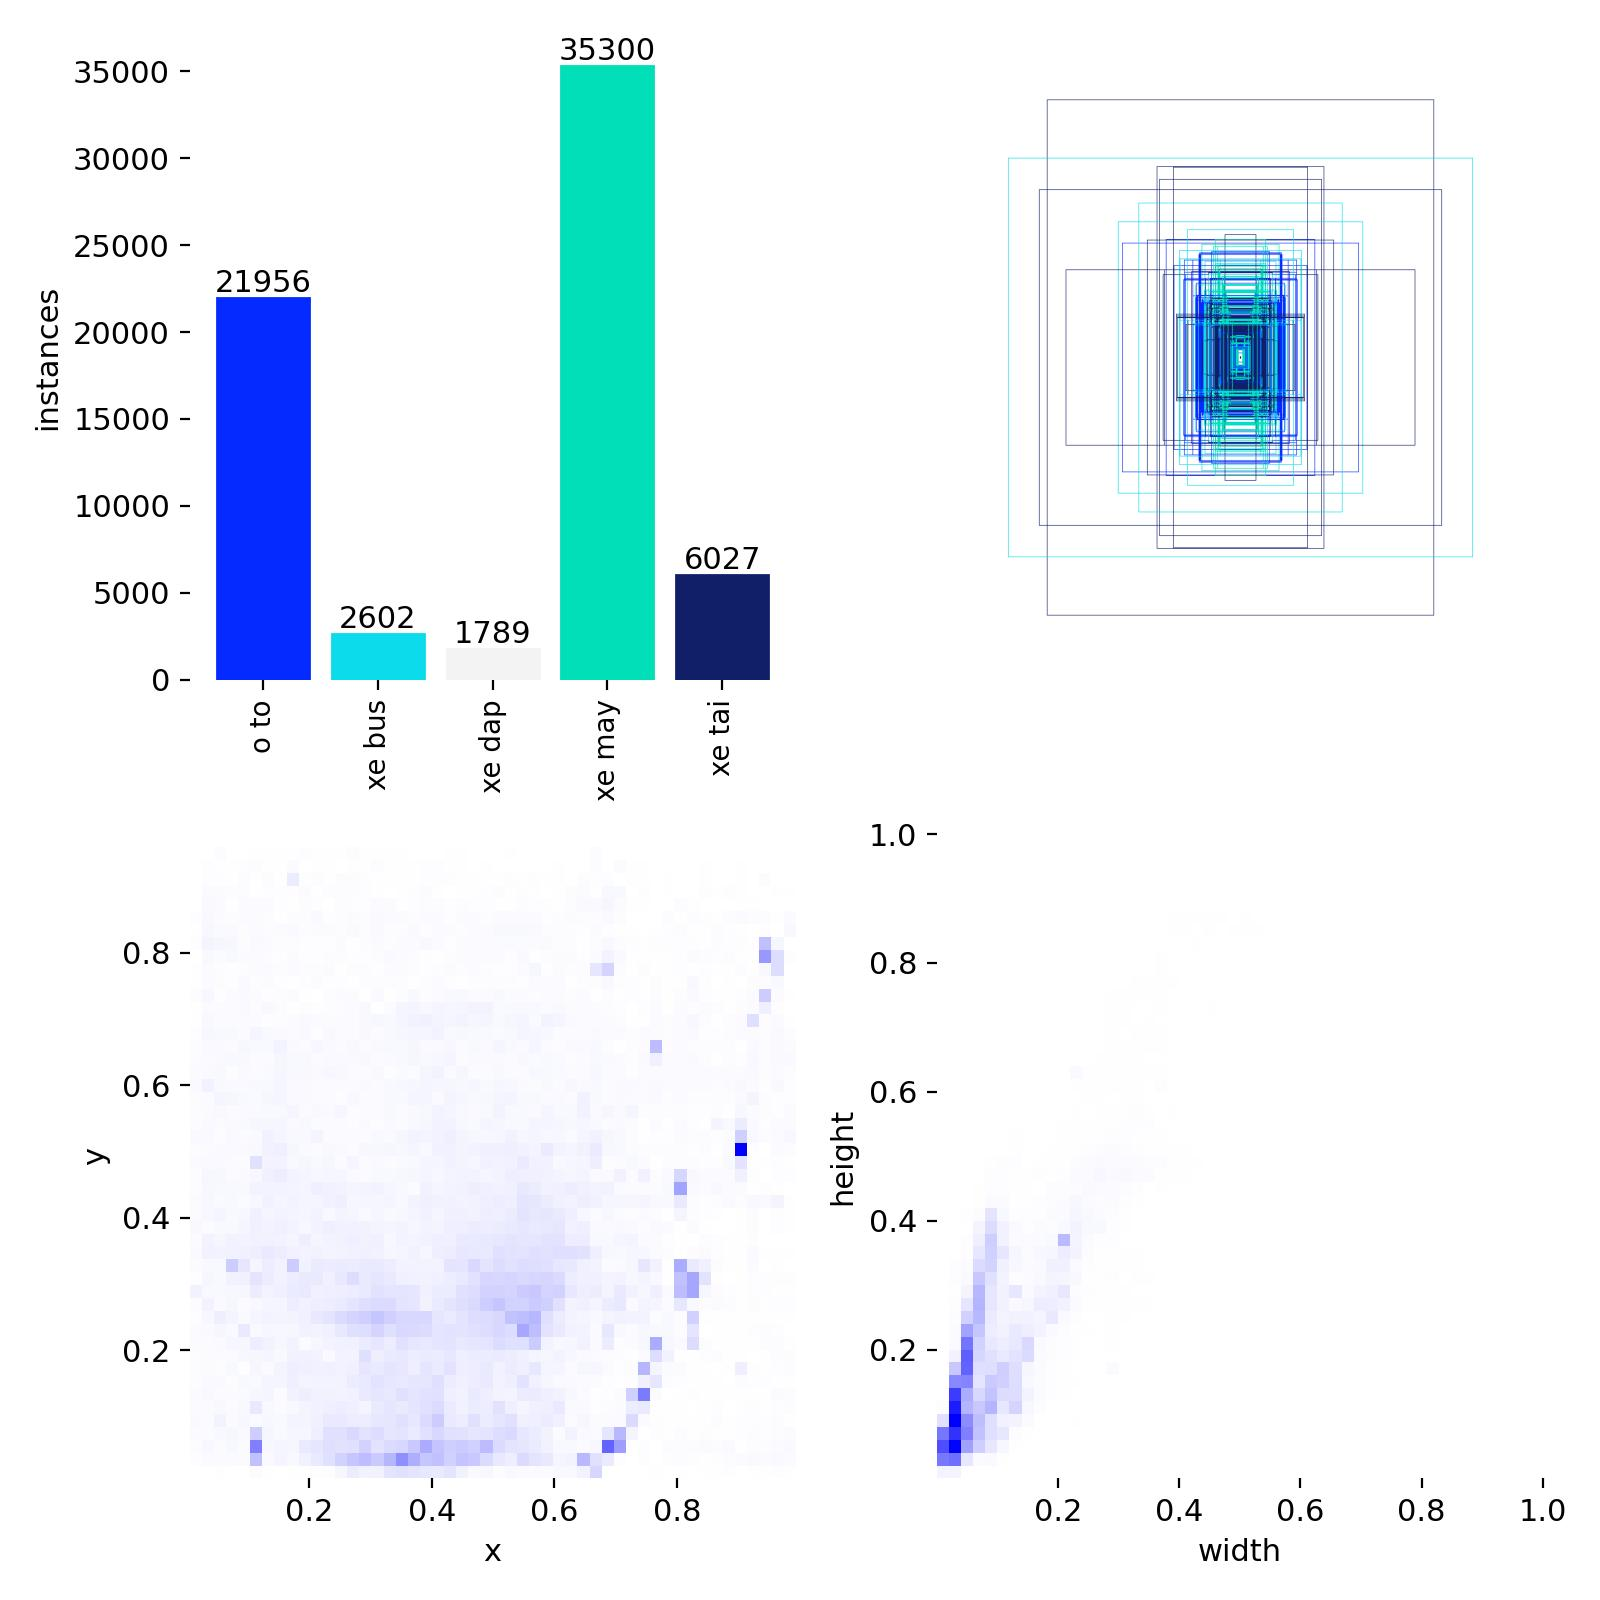
\includegraphics[width=0.7\linewidth]{Figures/labels.jpg}
    \caption{Phân bố số lượng nhãn và vị trí không gian của các đối tượng}
    \label{fig:labels_dist}
\end{figure}

\begin{itemize}
    \item \textbf{Quy mô:} Tổng cộng đã gán nhãn cho hơn \textbf{16.000 ảnh} với hơn \textbf{65.000 bounding boxes}.
    
    \item \textbf{Định dạng:} Nhãn được xuất ra dưới định dạng YOLO chuẩn, bao gồm 5 lớp đối tượng:
    \begin{enumerate}
        \item \textbf{xe may:} Bao gồm xe máy số, xe tay ga và xe máy điện (chiếm tỷ trọng lớn nhất).
        \item \textbf{o to:} Ô tô con, xe taxi, xe bán tải.
        \item \textbf{xe bus:} Xe buýt nội đô và xe khách.
        \item \textbf{xe tai:} Xe tải nhẹ và xe tải nặng.
        \item \textbf{xe dap:} Xe đạp và xe đạp điện.
    \end{enumerate}
\end{itemize}

Quy trình gán nhãn tuân thủ nguyên tắc: chỉ gán nhãn các đối tượng nhìn thấy rõ ít nhất 30\%, các đối tượng quá mờ hoặc bị che khuất quá nhiều sẽ được bỏ qua để tránh làm nhiễu mô hình.

Từ biểu đồ phân bố (Hình \ref{fig:labels_dist}), ta nhận thấy sự mất cân bằng dữ liệu đặc trưng: lớp 'Xe máy' và 'Ô tô' chiếm tỷ trọng lớn, trong khi 'Xe buýt' và 'Xe đạp' chiếm thiểu số. Kích thước bounding box tập trung nhiều ở vùng nhỏ và trung tâm, phản ánh các đối tượng xe cộ thường xuất hiện ở xa và đi vào giữa khung hình từ góc quay camera giám sát.

\subsection{Tiền xử lý dữ liệu}
Trước khi đưa vào huấn luyện, dữ liệu hình ảnh được xử lý qua các bước:

\begin{itemize}
    \item \textbf{Auto-Orientation:} Điều chỉnh hướng ảnh dựa trên thông tin EXIF.
    \item \textbf{Resize:} Đưa ảnh về kích thước tiêu chuẩn $416 \times 416$ pixels. Đây là kích thước tối ưu được chúng tôi lựa chọn để cân bằng giữa tốc độ xử lý và độ chính xác.
    \item \textbf{Augmentation:} Sử dụng kỹ thuật Mosaic Augmentation (ghép 4 ảnh huấn luyện thành 1) trong quá trình train của YOLOv8. Kỹ thuật này giúp mô hình học được các đối tượng ở nhiều tỷ lệ kích thước khác nhau và tăng khả năng nhận diện trong các ngữ cảnh phức tạp.
\end{itemize}

%============================================================
% PHẦN 2: HUẤN LUYỆN MÔ HÌNH PHÁT HIỆN PHƯƠNG TIỆN
%============================================================
\section{Huấn luyện mô hình phát hiện phương tiện}

\subsection{Cấu hình huấn luyện}
Chúng tôi sử dụng mô hình cơ sở (pre-trained) \texttt{yolov8n.pt} (phiên bản nano) được huấn luyện trước trên bộ dữ liệu COCO. Việc sử dụng Transfer Learning giúp mô hình hội tụ nhanh hơn và đạt độ chính xác tốt hơn với lượng dữ liệu giới hạn.

Các tham số huấn luyện chính được thiết lập như sau:

\begin{table}[!ht]
\centering
\caption{Tham số cấu hình huấn luyện YOLOv8 cho phát hiện phương tiện}
\label{tab:training_params_vehicle}
\begin{tabular}{|l|l|}
\hline
\textbf{Tham số} & \textbf{Giá trị} \\ \hline
Kích thước ảnh & 416 \\ \hline
Số lượng Epochs & 100 \\ \hline
Batch Size & 16 \\ \hline
Optimizer & SGD \\ \hline
Initial Learning Rate & 0.01 \\ \hline
Momentum & 0.937 \\ \hline
Weight Decay & 0.0005 \\ \hline
Số lớp & 5 (xe máy, ô tô, xe buýt, xe tải, xe đạp) \\ \hline
\end{tabular}
\end{table}

\subsection{Quá trình tối ưu hóa}
Trong quá trình huấn luyện, hàm mất mát tổng hợp bao gồm Box Loss, Class Loss và DFL Loss được theo dõi sát sao. Chúng tôi áp dụng kỹ thuật \textbf{Early Stopping} để dừng huấn luyện nếu chỉ số mAP@50 trên tập validation không cải thiện sau 50 epochs liên tiếp, nhằm tránh hiện tượng quá khớp (overfitting).

%============================================================
% PHẦN 3: THUẬT TOÁN XÁC ĐỊNH HƯỚNG DI CHUYỂN
%============================================================
\section{Thuật toán xác định hướng di chuyển}
\label{sec:direction_algo}

Khác với các phương pháp truyền thống chỉ dựa vào sự thay đổi tọa độ đơn thuần, hệ thống đề xuất sử dụng cơ chế Direction Fusion kết hợp hai nguồn thông tin để đạt độ chính xác cao nhất ngay cả khi camera bị nghiêng hoặc xe di chuyển phức tạp.

\subsection{Phân tích quỹ đạo với Reference Vector (Trajectory-based)}
Module \texttt{TrajectoryDirectionAnalyzer} xác định hướng di chuyển bằng cách so sánh vector chuyển động của xe với vector tham chiếu của đường. Phương pháp này giúp loại bỏ sai số do góc quay của camera.

\begin{enumerate}
    \item \textbf{Thiết lập Reference Vector ($\vec{V}_{ref}$):} Vector này được xác định thủ công hoặc tự động, đại diện cho hướng "đi thẳng" trên khung hình (ví dụ: vector dọc theo làn đường).
    
    \item \textbf{Tính toán Motion Vector ($\vec{V}_{motion}$):} Được tính từ $N$ vị trí lịch sử gần nhất của xe (sliding window size = 15).
    
    \item \textbf{Tính góc lệch tương đối ($\theta$):}
    Sử dụng tích vô hướng (Dot Product) và tích có hướng (Cross Product) để xác định góc lệch:
    \begin{equation}
        \theta = \text{atan2}(\vec{V}_{motion} \times \vec{V}_{ref}, \vec{V}_{motion} \cdot \vec{V}_{ref})
    \end{equation}
    Kết quả $\theta$ (đổi sang độ) được dùng để phân loại với ngưỡng 50°:
    \begin{itemize}
        \item $|\theta| \le 50^\circ$: Đi thẳng (STRAIGHT).
        \item $\theta > 50^\circ$: Rẽ phải (RIGHT).
        \item $\theta < -50^\circ$: Rẽ trái (LEFT).
    \end{itemize}
\end{enumerate}

\subsection{Xác định hướng dựa trên vùng quan tâm (ROI-based)}
Module \texttt{ROIDirectionManager} sử dụng các đa giác (polygons) được định nghĩa trước trên mặt đường. Khi trọng tâm của xe nằm trong vùng ROI nào, xe sẽ được gán nhãn hướng tương ứng của vùng đó (ví dụ: Làn rẽ trái, Làn đi thẳng). Phương pháp này hoạt động tốt ngay cả khi xe di chuyển chậm hoặc đứng yên chờ đèn.

\subsection{Cơ chế kết hợp (Direction Fusion)}
Module \texttt{DirectionFusion} tổng hợp kết quả từ hai nguồn trên để đưa ra quyết định cuối cùng, giải quyết bài toán xung đột dữ liệu:

\begin{algorithm}[!ht]
\SetAlgoLined
\KwIn{$D_{traj}$ (Trajectory Direction), $C_{traj}$ (Confidence), $D_{roi}$ (ROI Direction)}
\KwOut{$D_{final}$ (Final Direction)}

\uIf{$D_{roi}$ is None \textbf{and} $D_{traj}$ is Unknown}{
    \Return Unknown\;
}
\uElseIf{$D_{roi}$ exists \textbf{and} $D_{traj}$ is Unknown}{
    \Return $D_{roi}$\; \tcp*[r]{Fallback to ROI}
}
\uElseIf{Conflict exists ($D_{roi} \neq D_{traj}$)}{
    \eIf{$C_{traj} \ge 0.5$}{
        \Return $D_{traj}$\; \tcp*[r]{Trajectory priority if confident}
    }{
        \Return $D_{roi}$\; \tcp*[r]{ROI priority if trajectory noisy}
    }
}
\Else{
    \Return $D_{roi}$ (matches $D_{traj}$)\;
}
\caption{Thuật toán Direction Fusion}
\label{alg:fusion}
\end{algorithm}

%============================================================
% PHẦN 4: HỆ THỐNG PHÁT HIỆN VI PHẠM
%============================================================
\section{Hệ thống phát hiện vi phạm}
\label{sec:violation_logic}

Hệ thống sử dụng máy trạng thái (state machine) để kiểm tra vi phạm, đảm bảo mỗi phương tiện chỉ bị xử lý một lần tại thời điểm cắt qua vạch dừng.

\subsection{Quản lý tín hiệu đèn giao thông}
Module \texttt{TrafficLightManager} sử dụng không gian màu HSV để phát hiện trạng thái đèn. Các ngưỡng màu được tinh chỉnh để phân biệt rõ ba trạng thái:
\begin{itemize}
    \item \textbf{Đỏ:} Hue $\in [0, 10] \cup [160, 180]$.
    \item \textbf{Vàng:} Hue $\in [15, 35]$.
    \item \textbf{Xanh:} Hue $\in [40, 90]$.
\end{itemize}
Hệ thống phân biệt được 4 loại đèn: Đèn tròn, Đèn rẽ trái, Đèn rẽ phải và Đèn đi thẳng.

\subsection{Logic phát hiện vượt đèn đỏ}
Logic kiểm tra vi phạm (\texttt{ViolationChecker}) được kích hoạt khi sự kiện \textit{Stopline Crossing} xảy ra. Thuật toán kiểm tra tính hợp lệ dựa trên sự kết hợp giữa hướng di chuyển của xe và trạng thái của tất cả các đèn hiện có.

\begin{algorithm}[!ht]
\SetAlgoLined
\KwIn{Vehicle Direction $D_{veh}$, Traffic Lights $TLs$}
\KwOut{IsViolation, Reason}

$has\_green\_arrow \leftarrow$ False\;
$has\_red\_arrow \leftarrow$ False\;
$any\_red \leftarrow$ False\;

\ForEach{light in $TLs$}{
    \If{light.color is GREEN}{
        \If{light matches $D_{veh}$ (Arrow or Circle)}{
            $has\_green\_arrow \leftarrow$ True\;
        }
    }
    \If{light.color is RED}{
        $any\_red \leftarrow$ True\;
        \If{light explicitly forbids $D_{veh}$}{
            $has\_red\_arrow \leftarrow$ True\;
        }
    }
}

\uIf{$has\_green\_arrow$}{
    \Return \textbf{False} (Allowed)\;
}
\uElseIf{$has\_red\_arrow$}{
    \Return \textbf{True} (Explicit Prohibition)\;
}
\uElseIf{$any\_red$ \textbf{and not} $has\_green\_arrow$}{
    \Return \textbf{True} (Red Light Violation)\;
}
\Else{
    \Return \textbf{False} (No clear violation)\;
}
\caption{Logic kiểm tra vượt đèn đỏ}
\label{alg:violation_engine}
\end{algorithm}

\subsection{Logic phát hiện sai làn đường}
Module \texttt{LaneManager} kiểm tra vị trí tâm xe so với các đa giác làn đường đã định nghĩa.
\begin{itemize}
    \item Sử dụng thuật toán \texttt{pointInPolygon} (Ray Casting).
    \item Mỗi làn đường có danh sách \texttt{allowed\_labels} (ví dụ: \texttt{['car', 'bus']}).
    \item Nếu loại phương tiện của xe không nằm trong danh sách cho phép của làn đường hiện tại $\rightarrow$ Vi phạm sai làn.
\end{itemize}

\subsection{Điểm chạm tham chiếu (Reference Point)}
Khi tính toán vi phạm (dù là đè vạch dừng hay lấn làn), tuyệt đối không dùng tâm của Bbox. Cần sử dụng \textbf{trung điểm cạnh đáy} của Bbox – tương ứng với vị trí bánh xe chạm đất. Điều này giúp loại bỏ lỗi dương tính giả (false positive) khi xe nghiêng hoặc do góc quay camera.

\subsection{Ngưỡng dung sai}
Nên thiết lập vùng đệm an toàn. Ví dụ: Xe chỉ bị coi là vi phạm nếu điểm chạm lấn sang vùng cấm quá $10\text{--}15\%$, hoặc lấn quá một số pixel nhất định. Điều này giúp hệ thống "mềm dẻo" hơn trước các sai số do rung lắc camera hoặc bounding box bị lệch nhẹ.

%============================================================
% PHẦN 5: PIPELINE NHẬN DIỆN BIỂN SỐ (ALPR)
%============================================================
\section{Pipeline nhận diện biển số xe (ALPR)}

Chúng tôi đề xuất hai phương pháp tiếp cận để giải quyết bài toán phát hiện biển số:
\begin{enumerate}
    \item \textbf{Phương pháp 1 (Hai giai đoạn - Two Stage):} Sử dụng mô hình chuyên biệt để phát hiện biển số sau khi đã phát hiện phương tiện.
    \item \textbf{Phương pháp 2 (Một giai đoạn - One Stage):} Tích hợp nhãn biển số vào mô hình phát hiện phương tiện để phát hiện đồng thời cả xe và biển số.
\end{enumerate}

\subsection{Phương pháp 1: Mô hình phát hiện biển số chuyên biệt}

\subsubsection{Tổng quan Pipeline}
Hệ thống nhận diện biển số được xây dựng theo kiến trúc Two-Stage với các bước:

\begin{figure}[!htbp]
    \centering
    \begin{tikzpicture}[
        node distance=0.8cm,
        box/.style={rectangle, draw, rounded corners, minimum width=3.5cm, minimum height=1cm, align=center},
        arrow/.style={->, thick, >=stealth}
    ]
        % Nodes
        \node[box, fill=blue!20] (frame) {Frame từ Video};
        \node[box, fill=orange!20, below=of frame] (yolo) {YOLOv8\\Plate Detection};
        \node[box, fill=yellow!20, below=of yolo] (crop) {Crop vùng\\biển số};
        \node[box, fill=green!20, below=of crop] (clahe) {CLAHE +\\Sharpening};
        \node[box, fill=purple!20, below=of clahe] (ocr) {PaddleOCR};
        \node[box, fill=cyan!20, below=of ocr] (correct) {Character\\Correction};
        \node[box, fill=red!20, below=of correct] (vote) {Voting \&\\Lock};
        \node[box, fill=gray!20, below=of vote] (output) {Kết quả\\biển số};
        
        % Arrows
        \draw[arrow] (frame) -- (yolo);
        \draw[arrow] (yolo) -- (crop);
        \draw[arrow] (crop) -- (clahe);
        \draw[arrow] (clahe) -- (ocr);
        \draw[arrow] (ocr) -- (correct);
        \draw[arrow] (correct) -- (vote);
        \draw[arrow] (vote) -- (output);
    \end{tikzpicture}
    \caption{Pipeline xử lý nhận diện biển số xe}
    \label{fig:plate_pipeline}
\end{figure}

\subsubsection{Plate Detection với YOLOv8}
Chúng tôi huấn luyện mô hình YOLOv8n trên bộ dữ liệu VNLP (Vietnamese License Plate) với cấu hình:

\begin{table}[!ht]
\centering
\caption{Cấu hình huấn luyện Plate Detection}
\label{tab:plate_train_config}
\begin{tabular}{|l|c|}
\hline
\textbf{Tham số} & \textbf{Giá trị} \\ \hline
Base model & YOLOv8n (pretrained) \\ \hline
Input size & 416 × 416 \\ \hline
Batch size & 16 \\ \hline
Epochs & 100 \\ \hline
Optimizer & AdamW \\ \hline
Learning rate & 0.002 (cosine decay) \\ \hline
Số lớp & 1 (license\_plate) \\ \hline
\end{tabular}
\end{table}

\subsubsection{Bộ dữ liệu VNLP}
Bộ dữ liệu VNLP bao gồm các ảnh biển số xe Việt Nam được gán nhãn với định dạng YOLO:
\begin{itemize}
    \item Tổng số ảnh huấn luyện: ~5000 ảnh
    \item Đa dạng điều kiện: Ban ngày, ban đêm, góc nghiêng
    \item Các loại biển: Xe ô tô, xe máy, biển trắng, biển vàng
\end{itemize}

\subsection{Phương pháp 2: Tích hợp phát hiện đa lớp (Semi-supervised)}

Để tối ưu hóa thời gian xử lý và tận dụng ngữ cảnh xe, chúng tôi đề xuất phương pháp thứ hai: huấn luyện một mô hình duy nhất có khả năng phát hiện đồng thời phương tiện và biển số.

\subsubsection{Tổng quan Pipeline}

\begin{figure}[!htbp]
    \centering
    \begin{tikzpicture}[
        node distance=0.8cm,
        box/.style={rectangle, draw, rounded corners, minimum width=3.5cm, minimum height=1cm, align=center},
        arrow/.style={->, thick, >=stealth}
    ]
        % Nodes
        \node[box, fill=blue!20] (frame) {Frame từ Video};
        \node[box, fill=orange!20, below=of frame] (yolo) {YOLOv8 6-Class\\(Xe + Biển số)};
        \node[box, fill=green!20, below=of yolo, xshift=-2.5cm] (vehicle) {Vehicle\\Detection};
        \node[box, fill=green!20, below=of yolo, xshift=2.5cm] (plate) {Plate\\Detection};
        \node[box, fill=teal!20, below=of vehicle, yshift=-1.5cm] (match) {Matching\\Plate → Vehicle\\(Containment)};
        \node[box, fill=yellow!20, below=of match] (crop) {Crop vùng\\biển số};
        \node[box, fill=pink!20, below=of crop] (preprocess) {Tiền xử lý\\(CLAHE)};
        \node[box, fill=cyan!20, below=of preprocess] (ocr) {PaddleOCR};
        \node[box, fill=purple!20, below=of ocr] (validate) {Validation\\\& Retry};
        \node[box, fill=lime!20, below=of validate] (output) {Kết quả\\(Vehicle ID + Plate)};

        % Arrows
        \draw[arrow] (frame) -- (yolo);
        \draw[arrow] (yolo) -- (vehicle);
        \draw[arrow] (yolo) -- (plate);
        \draw[arrow] (vehicle) |- (match);
        \draw[arrow] (plate) |- (match);
        \draw[arrow] (match) -- (crop);
        \draw[arrow] (crop) -- (preprocess);
        \draw[arrow] (preprocess) -- (ocr);
        \draw[arrow] (ocr) -- (validate);
        \draw[arrow] (validate) -- (output);
    \end{tikzpicture}
    \caption{Pipeline Phương pháp 2: Phát hiện đồng thời xe và biển số trong một mô hình}
    \label{fig:alpr_method2_pipeline}
\end{figure}

Ưu điểm của phương pháp này:
\begin{itemize}
    \item \textbf{Hiệu quả:} Chỉ cần 1 lần forward pass qua YOLOv8 để có cả xe và biển số
    \item \textbf{Ngữ cảnh:} Mô hình học được mối quan hệ vị trí giữa xe và biển số
    \item \textbf{Tốc độ:} Giảm độ trễ inference so với phương pháp 2 giai đoạn
    \item \textbf{Mapping tự động:} Dễ dàng liên kết biển số với xe thông qua kiểm tra containment (biển số nằm 100\% trong bbox xe)
\end{itemize}

\subsubsection{Quy trình gán nhãn bán giám sát (Semi-supervised Labeling)}
Do bộ dữ liệu phương tiện gốc (\texttt{vietnam\_vehicle\_dataset}) chỉ chứa 5 nhãn phương tiện, chúng tôi thực hiện quy trình gán nhãn tự động để bổ sung nhãn biển số:

\begin{enumerate}
    \item \textbf{Bước 1 - Chuẩn bị mô hình Teacher:} Sử dụng mô hình phát hiện biển số (Model 1 - đã huấn luyện trên VNLP) làm nòng cốt.
    \item \textbf{Bước 2 - Inference gán nhãn:} Chạy Model 1 trên toàn bộ tập ảnh của \texttt{vietnam\_vehicle\_dataset}.
    \item \textbf{Bước 3 - Hợp nhất nhãn:} Bổ sung các bounding box biển số (license\_plate) vào các file annotation gốc. Nâng tổng số lớp từ 5 lên 6 (5 loại xe + license\_plate).
\end{enumerate}

\subsubsection{Huấn luyện mô hình tích hợp}
Sau khi có bộ dữ liệu 6 lớp, chúng tôi tiến hành huấn luyện lại từ đầu với cấu hình tương tự:
\begin{itemize}
    \item \textbf{Model:} YOLOv8n
    \item \textbf{Epochs:} 100
    \item \textbf{Image Size:} 416 pixel
    \item \textbf{Classes:} 6 (Xe máy, Xe đạp, Ô tô, Xe buýt, Xe tải, Biển số)
\end{itemize}

Phương pháp này giúp mô hình học được mối tương quan vị trí giữa xe và biển số, đồng thời giảm độ trễ inference (do chỉ cần 1 lần forward pass).

%============================================================
% PHẦN 6: TIỀN XỬ LÝ ẢNH BIỂN SỐ
%============================================================
\section{Tiền xử lý ảnh biển số}

Sau khi crop vùng biển số, chúng tôi áp dụng các bước tiền xử lý:

\subsection{Bước 1: CLAHE (Contrast Limited Adaptive Histogram Equalization)}
Áp dụng CLAHE để cải thiện độ tương phản của ảnh biển số:
\begin{itemize}
    \item Chuyển ảnh sang grayscale
    \item Áp dụng CLAHE với \texttt{clipLimit=2.0} và \texttt{tileGridSize=(8,8)}
    \item Chuyển lại về ảnh màu để đưa vào OCR
\end{itemize}

\subsection{Bước 2: Sharpening}
Áp dụng bộ lọc làm sắc nét để tăng cường cạnh của các ký tự, sử dụng kernel sharpening chuẩn:
\begin{equation}
K_{sharpen} = \begin{bmatrix}
0 & -1 & 0 \\
-1 & 5 & -1 \\
0 & -1 & 0
\end{bmatrix}
\end{equation}

%============================================================
% PHẦN 7: OCR VỚI PADDLEOCR
%============================================================
\section{OCR với PaddleOCR}

\subsection{Cấu hình PaddleOCR}
PaddleOCR được khởi tạo với các tham số:
\begin{itemize}
    \item \texttt{use\_angle\_cls=False}: Biển số đã được crop đúng hướng
    \item \texttt{lang='en'}: Ký tự biển số là alphanumeric
    \item \texttt{use\_gpu=True}: Tăng tốc với GPU
\end{itemize}

\subsection{Character Correction}
Do PaddleOCR có thể nhầm lẫn một số ký tự tương tự, chúng tôi áp dụng bước hiệu chỉnh:

\begin{table}[!ht]
\centering
\caption{Bảng hiệu chỉnh ký tự}
\label{tab:char_correction}
\begin{tabular}{|c|c|l|}
\hline
\textbf{Sai} & \textbf{Đúng} & \textbf{Giải thích} \\ \hline
0 (số) & O (chữ) & Vị trí chữ cái (index 2) \\ \hline
O (chữ) & 0 (số) & Vị trí chữ số \\ \hline
1 (số) & I (chữ) & Hiếm gặp \\ \hline
8 (số) & B (chữ) & Vị trí chữ cái \\ \hline
\end{tabular}
\end{table}

Logic hiệu chỉnh dựa trên định dạng biển số Việt Nam:
\begin{itemize}
    \item Vị trí 0-1: Chữ số (mã tỉnh)
    \item Vị trí 2: Chữ cái (seri)
    \item Vị trí 3-7: Chữ số (số thứ tự)
\end{itemize}

%============================================================
% PHẦN 8: VALIDATION & RETRY MECHANISM
%============================================================
\section{Validation \& Retry Mechanism}

\subsection{Vấn đề}
OCR có thể cho kết quả khác nhau giữa các frame do:
\begin{itemize}
    \item Biển số bị rung, blur
    \item Ánh sáng thay đổi
    \item Góc nhìn thay đổi khi xe di chuyển
    \item Nhiễu từ mô hình OCR
\end{itemize}

\subsection{Giải pháp: Format Validation}
Thay vì sử dụng voting mechanism phức tạp, chúng tôi áp dụng validation dựa trên format chuẩn biển số Việt Nam:
\begin{itemize}
    \item \textbf{Xe máy} (cls\_id 2, 3): Format xxYZxxxxx (8-9 ký tự)
    \begin{itemize}
        \item xx: 2 chữ số đầu (mã tỉnh)
        \item Y: 1 chữ cái (seri)
        \item Z: 1 chữ số hoặc chữ cái
        \item xxxxx: 4-5 chữ số cuối
        \item Ví dụ: \texttt{29B12345}, \texttt{30M04019}
    \end{itemize}
    \item \textbf{Ô tô} (cls\_id 0, 1, 4): Format xxYxxxxx (7-8 ký tự)
    \begin{itemize}
        \item xx: 2 chữ số đầu (mã tỉnh)
        \item Y: 1 chữ cái (seri)
        \item xxxxx: 4-5 chữ số cuối
        \item Ví dụ: \texttt{51A1234}, \texttt{30H12345}
    \end{itemize}
\end{itemize}

\subsection{Retry Mechanism}
Khi OCR không cho kết quả hợp lệ, hệ thống tự động retry:
\begin{itemize}
    \item Chỉ lưu kết quả \textbf{đúng format} (validated)
    \item Nếu OCR trả về text không khớp pattern $\rightarrow$ không lưu, thử lại frame tiếp theo
    \item Nếu đã có kết quả hợp lệ $\rightarrow$ dừng OCR cho xe đó (tiết kiệm tài nguyên)
    \item Log chi tiết: \texttt{VALID}, \texttt{INVALID FORMAT}, \texttt{NO TEXT}
\end{itemize}

Điều này giúp:
\begin{itemize}
    \item Loại bỏ kết quả nhiễu ngay từ đầu
    \item Đảm bảo chỉ hiển thị biển số đúng format
    \item Giảm độ phức tạp so với voting mechanism
    \item Tận dụng khả năng tracking để retry tự động
\end{itemize}

%============================================================
% PHẦN 9: TÍCH HỢP VỚI VEHICLE TRACKING
%============================================================
\section{Tích hợp với Vehicle Tracking}

Pipeline biển số được tích hợp với hệ thống tracking để:
\begin{itemize}
    \item Chỉ xử lý OCR cho xe có \texttt{track\_id} mới hoặc chưa có kết quả valid
    \item Liên kết biển số với từng xe cụ thể thông qua track\_id
    \item Tự động dừng OCR khi đã có kết quả đúng format để tiết kiệm tài nguyên
    \item Sử dụng format validation để đảm bảo chất lượng kết quả
\end{itemize}

\section{Tổng kết phương pháp}

Hệ thống hoàn chỉnh được xây dựng với các thành phần chính:

\begin{enumerate}
    \item \textbf{Detection:} YOLOv8n cho cả phương tiện (5 lớp) và biển số (1 lớp)
    \item \textbf{Tracking:} ByteTrack với Kalman Filter để theo dõi liên tục
    \item \textbf{Direction Analysis:} Direction Fusion kết hợp Trajectory + ROI
    \item \textbf{Violation Detection:} State machine với logic đèn + làn đường
    \item \textbf{ALPR:} PaddleOCR với Character Correction + Voting \& Lock
\end{enumerate}

Toàn bộ pipeline được tích hợp trong ứng dụng PyQt5 với giao diện đồ họa thân thiện, cho phép người dùng cấu hình ROI, vạch dừng, làn đường một cách trực quan.

